\hypertarget{okno__glowne_8cpp}{}\section{Dokumentacja pliku okno\+\_\+glowne.\+cpp}
\label{okno__glowne_8cpp}\index{okno\+\_\+glowne.\+cpp@{okno\+\_\+glowne.\+cpp}}


Zawiera definicje metod klasy \hyperlink{class_okno_glowne}{Okno\+Glowne}.  


{\ttfamily \#include \char`\"{}okno\+\_\+glowne.\+hh\char`\"{}}\\*
Wykres zależności załączania dla okno\+\_\+glowne.\+cpp\+:
\nopagebreak
\begin{figure}[H]
\begin{center}
\leavevmode
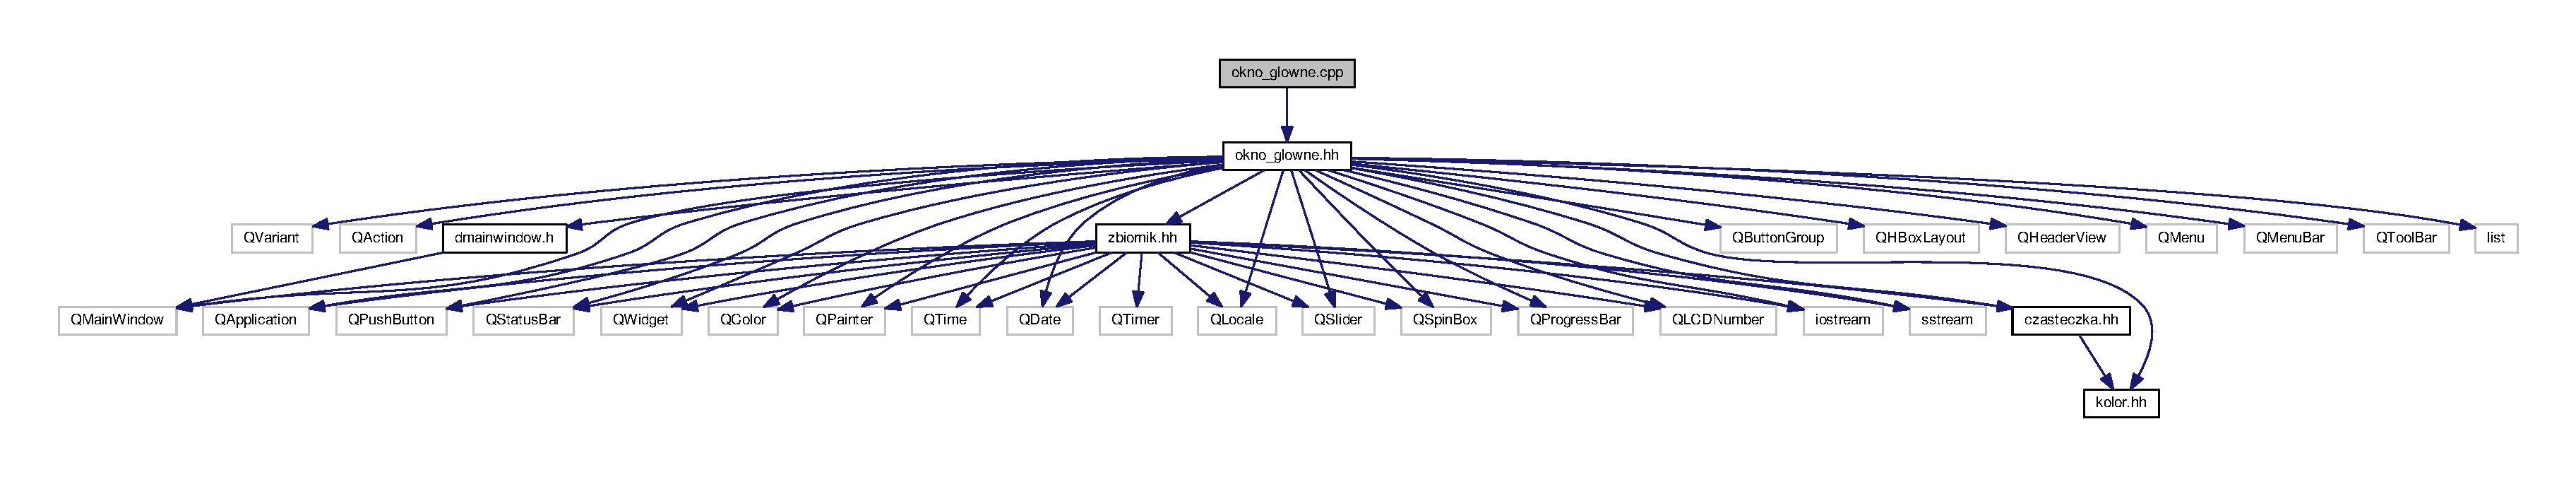
\includegraphics[width=350pt]{okno__glowne_8cpp__incl}
\end{center}
\end{figure}


\subsection{Opis szczegółowy}
W pliku znajduja sie\+:
\begin{DoxyItemize}
\item definicje konstruktorow, metod i przeciazen klasy \hyperlink{class_okno_glowne}{Okno\+Glowne}. 
\end{DoxyItemize}